\begin{titlepage}
    \centering
    \vspace*{2cm}
    
    {\Huge\textbf{Libreria AstDyn}}\\[1cm]
    {\Large\textit{Manuale Scientifico}}\\[0.5cm]
    {\large Meccanica Celeste e Determinazione Orbitale}\\[2cm]
    
    \begin{figure}[H]
        \centering
        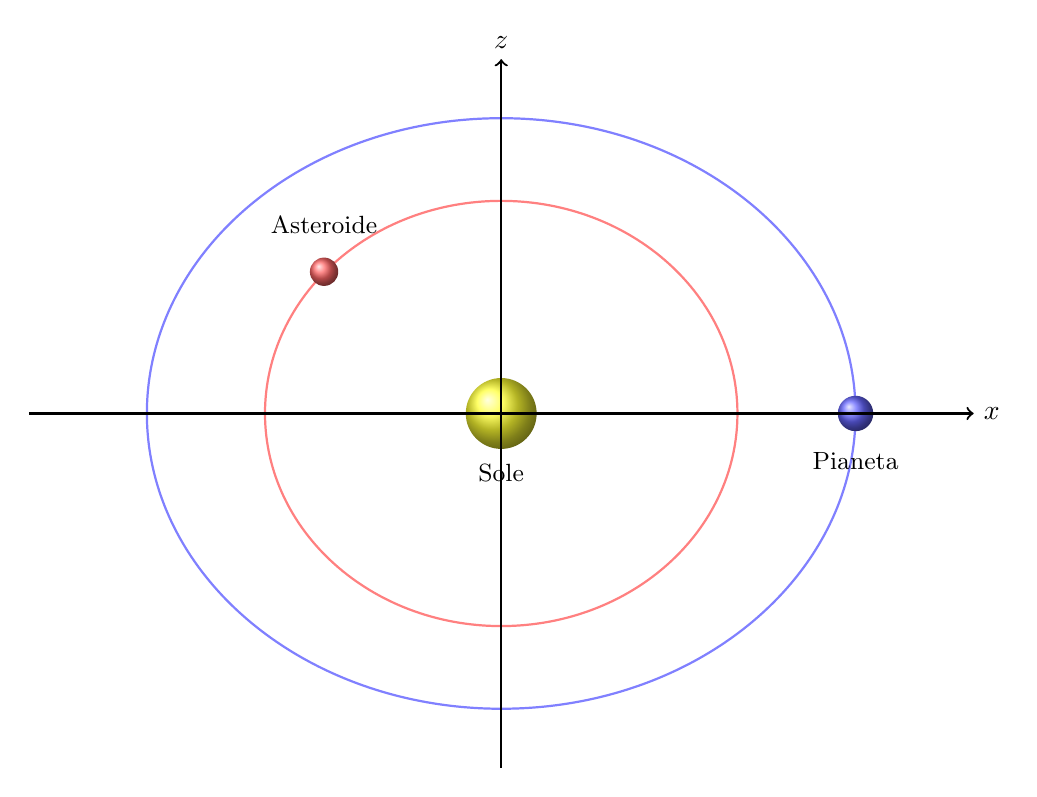
\begin{tikzpicture}[scale=1.5]
            % Sole al centro
            \shade[ball color=yellow!80] (0,0) circle (0.3);
            
            % Orbite
            \draw[thick,blue!50] (0,0) ellipse (3 and 2.5);
            \draw[thick,red!50] (0,0) ellipse (2 and 1.8);
            
            % Pianeti
            \shade[ball color=blue!60] (3,0) circle (0.15);
            \shade[ball color=red!60] (-1.5,1.2) circle (0.12);
            
            % Assi coordinati
            \draw[->,thick] (-4,0) -- (4,0) node[right] {$x$};
            \draw[->,thick] (0,-3) -- (0,3) node[above] {$z$};
            
            % Etichette
            \node at (3,-0.4) {\small Pianeta};
            \node at (-1.5,1.6) {\small Asteroide};
            \node at (0,-0.5) {\small Sole};
        \end{tikzpicture}
        \caption*{Dinamica orbitale eliocentrica}
    \end{figure}
    
    \vfill
    
    {\Large\textbf{Michele Bigi}}\\[0.5cm]
    {\large Versione 1.0.0}\\[0.3cm]
    {\large\today}\\[1cm]
    
    \vspace{1cm}
    
    \begin{minipage}{0.8\textwidth}
        \centering
        \small
        \textit{Una libreria completa in C++17 per la meccanica celeste,\\
        la determinazione orbitale e i calcoli di astrodinamica}
    \end{minipage}
    
\end{titlepage}

\clearpage
